\documentclass{beamer}
\usepackage[francais]{babel}
\usepackage[utf8]{inputenc} % Required for including letters with accents
\usepackage[T1]{fontenc} % Use 8-bit encoding that has 256 glyphs
\usepackage{pythontex}
\usepackage{amsthm}
\usepackage{amsmath}
\usepackage{amssymb}
\usepackage{mathrsfs}
\usepackage{graphicx}
\usepackage{geometry}
\usepackage{stmaryrd}
\usepackage{tikz}
\usetikzlibrary{patterns}
%\usetikzlibrary{intersections}
% Code syntax highlighter
\usepackage[cache=false]{minted}

\usepackage{stmaryrd}
%\usepackage{tikz}
%\usetikzlibrary{tikzmark}
\usepackage{empheq}
\usepackage{longtable}
\usepackage{booktabs} 
\usepackage{array}
\usepackage{pstricks}
\usepackage{pst-3dplot}
\usepackage{pst-tree}
\usepackage{pstricks-add}
\usepackage{upgreek}
%\usepackage{epstopdf}
\usepackage{eolgrab}
\usepackage{chngpage}
 \usepackage{calrsfs}
 % Appel du package pythontex 
\usepackage{pythontex}

\usetikzlibrary{decorations.pathmorphing}
\def \de {{\rm d}}
%\usepackage{color}
%\usepackage{xcolor}
%\usepackage{textcomp}
\newcommand{\mybox}[1]{\fbox{$\displaystyle#1$}}
\newcommand{\myredbox}[1]{\fcolorbox{red}{white}{$\displaystyle#1$}}
\newcommand{\mydoublebox}[1]{\fbox{\fbox{$\displaystyle#1$}}}
\newcommand{\myreddoublebox}[1]{\fcolorbox{red}{white}{\fcolorbox{red}{white}{$\displaystyle#1$}}}
\usetheme[options]{Boadilla}
\definecolor{purple2}{RGB}{153,0,153} % there's actually no standard purple
\definecolor{green2}{RGB}{0,153,0} % a darker green
\usepackage{xcolor}

\definecolor{LightGray}{gray}{0.9}
%\usepackage{listings}

  \title{Équations différentielles  ordinaires (EDO)}
  \author{ \textsc{Ibrahim ALAME}}\institute{ESTP}
\date{23/01/2024}
  \begin{document}

 \begin{frame}
 \begin{center}
 Chapitre 2
 \end{center}
  \titlepage
  \end{frame}

 \begin{frame}
  \frametitle{Equations différentielles}
  \begin{block}{Problème de Cauchy}
  \[\myredbox{(\star)\left\{\begin{array}{l}
{\bf y}'(t) = {\bf f}(t; {\bf y}(t)) \mbox{ dans }I\\
{\bf y}(t_0) = {\bf y}_0
\end{array}\right.
}\]
\begin{itemize}
\item  $I$ un intervalle de $\mathbb{R}$
\item ${\bf f}$ une fonction à deux variables de $I\times \mathbb{R}^n$ dans $\mathbb{R}^n$. 
\item ${\bf y}:I\to \mathbb{R}^n$ la fonction inconnue.
\item $t_0(=0)$ est un point de $I$. 
\end{itemize}
  \end{block}
  \[\left\{\begin{array}{l}
  y'_1(t)=f_1(t,y_1(t),y_2(t),...y_n(t))\\
  y'_2(t)=f_2(t,y_1(t),y_2(t),...y_n(t))\\
  \cdots\cdots \\
  y'_n(t)=f_n(t,y_1(t),y_2(t),...y_n(t))
  \end{array}\right.\]


  \end{frame}
  
   \begin{frame}
  \frametitle{Quelques exemples}
  
\begin{itemize}
\item  $y' = y + 1$ est une équation différentielle linéaire du premier
ordre. En se limitant à l'intervalle $[0; 5]$ et avec la condition
$y(0) = 3$, on a un problème de Cauchy.
\item $\left\{\begin{array}{l}
x' = x + y + t\\
y' = 2x - 3y + t^2
\end{array} \right.$
 est un système différentiel à deux inconnues du premier ordre. On se ramène à la forme générale $Y' = F(t; Y)$ en posant une fonction inconnue vectorielle
\[Y (t) =\left(\begin{array}{l}
x(t)\\
y(t)
\end{array} \right)\]
\item Pour une équation différentielle du second ordre comme $y'' + y' + y = t $ on peut se ramener à la forme présentée en posant une fonction inconnue vectorielle 
\[Y (t) =\left(\begin{array}{l}
y'(t)\\
y(t)
\end{array} \right)\]
\end{itemize}
 
  \end{frame}
  
  
  \begin{frame}
Une équation différentielle d'ordre $p$ de la forme 
\[y^{(p)}=f(t,y,y',\cdots,y^{(p-1)})\] 
où $p > 1$ se ramène à un système équivalent en posant :
 \[\left\{\begin{array}{l}
  z'_1(t)=z_2(t)\\
  z'_2(t)=z_3(t)\\
  \cdots\cdots \\
  z'_p(t)=f(t,z_1(t),z_2(t),...z_{p-1}(t))
  \end{array}\right.\]

autrement dit :
\[{\bf z}'(t) = {\bf F}(t; {\bf z}(t)) \]
\begin{block}{Exemple}
\[y''(t)-ay'(t)-by(t)=f(t)\]
On pose $z_1=y$ et $z_2=y'$ d'où le système

 \[\left\{\begin{array}{l}
  z'_1(t)=z_2(t)\\
  z'_2(t)= b z_1(t)+a z_2(t)+f(t)
  \end{array}\right.\]
\end{block}

  \end{frame}
  \begin{frame}
    \begin{theorem}[de Cauchy-Lipschitz]
    Soit $f$ une application continue : \[f:(t,{\bf z})\in(0,T)\times \mathbb{R}^n\mapsto f(t,{\bf z})\in \mathbb{R}^n\]
Si $f$ vérifie la condition de Lipschitz,
\[\forall t\in[0,T], \quad \forall |z_1|, |z_2| \in \mathbb{R}^n, \quad \|f(t, z_1) - f(t, z_2)\| \leq L\|z_1 - z_2\| \]
alors il y a existence et unicité locale de la solution du problème de Cauchy.
\end{theorem}
    Le théorème est admis dans ce cours, il s'obtient via un argument de point fixe pour les applications contractantes dans l'espace de Banach...

   \end{frame}
   
  \begin{frame} 
Nous considérons maintenant trois exemples typiques:
\begin{itemize}
\item $y'(t) = a y(t)$
 \[f(t,y) = a y \Longrightarrow |f(t, y_1) - f(t, y_2)|=a|y_1 - y_2|\]
\item $y'(t) = \left[y(t)\right]^2$. 

Nous vérifions facilement que $f(t,y) = y^2$ est localement lipschitzienne car $f$ est de classe $C^1$ donc localement lipschitzienne d'après  le Théorème des accroissements
fnis.
\item $y'(t) = \sqrt[3]{y(t)}$. 

La fonction  $f(t,y)=\sqrt[3]{y(t)}$ n'est pas lipschitzienne car elle n'est pas dérivable en $0$ et donc le théorème ne s'applique pas!
\end{itemize}  
 
    \end{frame} 
%%%%%%%%%%%%%%%%%%%%%%%%%%%%%%%%%%%%%%%%%%%%%%%%%%%%%%    
\begin{frame}   
\frametitle{Méthodes numériques} 
   On va s'intéresser à différentes méthodes numériques de calcul d'approximations de solutions d'équations (ou de systèmes) différentielles. Plus précisément de résolution de problèmes de Cauchy (une équation assortie d'une condition initiale garantissant
l'unicité de la solution). 
 \end{frame}   
%%%%%%%%%%%%%%%%%%%%%%%%%%%%%%%%%%%%%%%%%%%%%%%%%%%%%%    
 %%%%%%%%%%%%%%%%%%%%%%%%%%%%%%%%%%%%%%%%%%%%%%%%%%%%%%    
\begin{frame}   
\frametitle{Principe} 
   On subdivise l'intervalle $[a; b]$ en $n$ intervalles de longueur $h$:
   \begin{center}
 \begin{tikzpicture}[domain=0:5]
  \draw[->] (-0.1,0) -- (6.1,0)  node[right] {$\scriptstyle t$};
  %\draw[->] (0,-0.1) -- (0,3.5) node[above] {$\scriptstyle y$};
  \path[fill=black]  (0,0) circle (.4mm) [fill=orange] node[below] {$\scriptstyle a=t_0$};
 \path[fill=black]  (1,0) circle (.4mm) [fill=orange];
 \path[fill=black]  (2,0) circle (.4mm) [fill=orange] node[below] {$\scriptstyle t_{i}$};
 \path[fill=black]  (3,0) circle (.4mm) [fill=orange];
   \draw  (2.5,0.5) node {$\scriptstyle h=\frac {b-a}n$};
   \draw[<->] (2,0.2) -- ++(1,0) ;
   \path[fill=black]  (4,0) circle (.4mm) [fill=orange];
    \path[fill=black]  (5,0) circle (.4mm) [fill=orange] node[below] {$\scriptstyle b=t_n$};

\end{tikzpicture}
 \end{center}
 \begin{itemize}
\item On a obtenu des nœuds $t_i$, $0\leq i\leq n$. ($n + 1$ nœuds).
\item On cherche à calculer des quantités $y_i$, une valeur approchée
de la vraie valeur $y(t_i)$ de la solution du problème de Cauchy,
que l'on ne connait pas.
 \end{itemize}
 
 \end{frame}   
%%%%%%%%%%%%%%%%%%%%%%%%%%%%%%%%%%%%%%%%%%%%%%%%%%%%%%    
 \begin{frame}  
 \frametitle{La méthode d'Euler}  
 Problème de Cauchy:
   \[\myredbox{(\star)\left\{\begin{array}{l}
{\bf y}'(t) = {\bf f}(t; {\bf y}(t)) \mbox{ dans }I\\
{\bf y}(t_0) = {\bf y}_0
\end{array}\right.
}\]
On cherche à approcher $ y(t_i) \simeq y_i $. Taylor à l'ordre 1:

\[y(t_i+h)=y(t_i)+hy'(t_i)+o(h)\mbox{ où } h=t_{i+1} - t_i = \frac Tn \]
or $y'(t_i)=f(t_i,y(t_i))$ d'où "l'idée" de considérer le schéma suivant:
\\
\\
Schéma d'Euler explicite:
\[\myredbox{\left\{\begin{array}{l}
y_{i+1}=y_i+h f(t_i,y_i) \\
y_0=y(0)

\end{array}\right.}
\]

 \end{frame}  
%%%%%%%%%%%%%%%%%%%%%%%%%%%%%%%%%%%%%%%%%%%%%%%%%%%%%%%%  

\begin{frame}    
   \frametitle{Un exemple (trop ?) élémentaire}
On considère le problème de Cauchy sur $I = [0; 1]$ décrit par l'équation $y' = y$ et $y(0) = 1$.
On subdivise $I$ en $n$ intervalles de longueur $h =\frac 1n$.

Ici $f (t; y) = y$. Le schéma d'Euler explicite s'écrit donc
\[y_{i+1} = y_i + hy_i = (1 + h)y_i\]
Pour tenir compte de la condition initiale, on a $y_0 = 1$.

On peut écrire ici $y_k = (1 + h)^ky_0 = (1 + h)^k$.
 \end{frame}  
%%%%%%%%%%%%%%%%%%%%%%%%%%%%%%%%%%%%%%%%%%%%%%%%%%%%%%%%  
\begin{frame}    
\frametitle{Un exemple (trop ?) élémentaire}
On peut aussi résoudre explicitement le problème de Cauchy qui a pour solution $y(t) = e^t$ .
On peut se demander si $y_k$ approche bien $y(t_k) = e^{kh}$.
On est amené à majorer $|y(t_k) - y_k|$ pour $k$ vérifiant $0\leq k \leq n$.
On obtient
\[\max_{0\leq k \leq n}|y(t_k) - y_k|\leq \frac e2h\]

On dira, pour cet exemple, que la méthode d'Euler explicite converge (l'erreur tend vers $0$ lorsque $n\to\infty$ ou, ce qui est équivalent, lorsque $h\to 0$ ).
 \end{frame}  
%%%%%%%%%%%%%%%%%%%%%%%%%%%%%%%%%%%%%%%%%%%%%%%%%%%%%%%%  
    
  \begin{frame}    
   \frametitle{La méthode d'Euler}


  \frametitle{La méthode d'Euler}
   \begin{center}
 \begin{tikzpicture}[domain=0:5]
  \draw[->] (-0.1,0) -- (6.1,0)  node[right] {$\scriptstyle t$};
  \draw[->] (0,-0.1) -- (0,3.5) node[above] {$\scriptstyle y$};
  \path[fill=black]  (0,0) circle (.4mm) [fill=gray] node[below] {$\scriptstyle 0=t_0$};
 \path[fill=black]  (1,0) circle (.4mm) [fill=gray];
 \path[fill=black]  (2,0) circle (.4mm) [fill=gray] node[below] {$\scriptstyle t_{i}$};
 \path[fill=black]  (3,0) circle (.4mm) [fill=gray];
   \draw  (2.5,0.5) node {$\scriptstyle h=\frac Tn$};
   \draw[<->] (2,0.2) -- ++(1,0) ;
   \path[fill=black]  (4,0) circle (.4mm) [fill=gray];
    \path[fill=black]  (5,0) circle (.4mm) [fill=gray] node[below] {$\scriptstyle T=t_n$};
\draw [domain=0:5][line width=0.5] plot(\x,{(1/3*\x*\x*\x-3*\x*\x+8*\x)/3});


 \draw[orange,dotted] (1,1.777)--(1,2.67);
 \draw[orange,dotted] (2,2.222)--(2,3.67);
  \draw[orange,dotted] (3,2)--(3,3.67);
  \draw[orange,dotted] (4,1.666)--(4,3.33);
  \draw[orange,dotted] (5,1.777)--(5,3.33); 
 \draw [domain=0:1,very thin, green][line width=0.5] plot(\x,{8/3*\x});
 \draw [domain=1:2, green] plot(\x,{7/9+\x});
   \draw [domain=2:3, green] plot(\x,{20/9});
 \draw [domain=3:4, green] plot(\x,{3-1/3*\x});
  \draw [domain=4:5, green] plot(\x,{16/9});
 \draw[orange] (0,0) --  (1,2.67)-- (2,3.67)--(3,3.67)--(4,3.33)--(5,3.33);
  \path[fill=black]   (1,2.67) circle (.4mm) [fill=blue];
  \path[fill=black]   (2,3.67) circle (.4mm) [fill=blue];
  \path[fill=black]  (3,3.67)circle (.4mm) [fill=blue];
  \path[fill=black]   (4,3.33) circle (.4mm) [fill=blue];
  \path[fill=black]  (5,3.33) circle (.4mm) [fill=blue];
  \draw[<->,very thin, blue] (2,2.22) -- (2,2.777);
   \draw (1.9,2.44) node{$\scriptstyle \varepsilon_i$};
 \draw[<->,very thin, blue] (2.1,2.22) -- (2.1,3.67);
   \draw (2.25,2.9) node{$\scriptstyle e_i$};    
   
\end{tikzpicture}
 \end{center}



\begin{itemize}
      \item  $e_i=y(t_i)-y_i$ l'erreur commise au point $t_i$
      \item  $\varepsilon_{i+1}=y(t_{i+1})-y(t_i)-h f(t_i,y(t_i))$ l'erreur de consistance,  c'est l'erreur systématique commise sur $y_{i+1}$ : c'est l'erreur de passage de 
 la valeur à l'instant $t_i$ supposée exacte à la valeur approchée en $t_{i+1}$.
      \end{itemize}

 \end{frame}  
%%%%%%%%%%%%%%%%%%%%%%%%%%%%%%%%%%%%%%%%%%%%%%%%%%%%%%%%      
           
      \begin{frame}
      \frametitle{Etude de l'erreur}
 On a     

 \[\begin{array}{ccl}
\left|e_{i+1}\right|&=&\left|y(t_{i+1})-y_{i+1}\right|\\
       &=&\left|\textcolor{orange}{ y(t_{i+1})-y(t_{i})-h f(t_i,y(t_i))}\right.\\
       &  & +\textcolor{cyan}{y(t_{i})}+h\textcolor{violet}{ f(t_i,y(t_i))} \\
       &  & \textcolor{cyan}{-y_i}+\textcolor{gray}{ y_i}\\
       &  & +\textcolor{gray}{hf(t_i,y_i)}-h\textcolor{violet}{f(t_i,y_i)}\\
       &  &\left. \textcolor{gray}{-y_{i+1} }\right|\\
       &\leq & \left|\textcolor{orange}{\varepsilon_{i+1}}\right|+\left|\textcolor{cyan}{e_{i}}\right|+h\left|\textcolor{violet}{f(t_i,y(t_i))-f(t_i,y_i)}\right|
\end{array}
\]
Si $f$ est lipschitzienne en $y$:
\[\myredbox{\left|e_{i+1}\right|\leq \left|\varepsilon_{i+1}\right|+(1+L h)\left|e_{i}\right|}\]

      \end{frame}
   
 \begin{frame}
 d'autre part
\[\begin{array}{ccl}
\left|\varepsilon_{i+1}\right|&=&\left|y(t_{i+1})-y(t_{i})-h f(t_i,y(t_i))\right|\\
&=&\left| \int_{t_i}^{t_{i+1}}y'(s)\de s- \int_{t_i}^{t_{i+1}}f(t_i,y(t_i))\de s\right|\\
&=&\left| \int_{t_i}^{t_{i+1}}(y'(s)-y'(t_i))\de s\right|\\
&\leq & M\cdot \frac{h^2}2
\end{array}
\]
où $\displaystyle M=\sup_{[0,T]}|f''|$.
Finalement
\[\myredbox{\left|e_{i+1}\right|\leq (1+L h)\left|e_{i}\right|+ M \cdot \frac{h^2}2}\]
\end{frame}   
   
 \begin{frame}
 
 \begin{block}{Lemme}
 Soit $(\theta_i)_i$ une suite de nombres positifs satisfaisant:
\[\theta_{i+1}\leq (1+A)\theta_i +B\]
où $A$ et $B$ sont des constantes strictement positives alors:
\[\theta_i \leq \exp(i A)\theta_0 +\frac{\exp(i A)- 1}{A}B\]
 \end{block}

Démonstration par récurrence.
Grâce au lemme, on a:
\[|e_i| \leq \exp(i L h)|e_0| +\frac{\exp(i L h)- 1}{L h}\cdot M\frac{h^2}2\]
or $e_0=0$ d'où le théorème:
\end{frame}   
   %%%%%%%%%%%%%%%%%%%%%%%%%%%%%%%%%%%%%%%%%%%%%%%%%%%%%%%%      
\begin{frame}
\frametitle{Estimation de l'erreur (Euler explicite)}
\begin{block}{Théorème (convergence et erreur pour Euler explicite)}
Supposons que les conditions du théorème de Cauchy-Lipschitz soient satisfaites ($f$ est $L$-lipschitzienne) , avec $y$ une solution de classe $\mathcal{C}^2$.

On note $e_k = y(t_k) - y-k$ et $M = \sup_{t\in I} |y''(t)|$.

On a la majoration pour $0\leq k \leq n$:
\[|e_k|\leq \frac{e^{khL}-1}{2L}M h\]
Donc
\[\myredbox{\max_{0\leq i\leq N}|e_i|\leq \frac{\exp(L T)- 1}{2L }Mh}\]
Et
\[\lim_{n\to\infty}\max_{0\leq k \leq n}|e_k|=0\]
\end{block}
 \end{frame}  
    %%%%%%%%%%%%%%%%%%%%%%%%%%%%%%%%%%%%%%%%%%%%%%%%%%%%%%%%      
\begin{frame}
à partir de ce théorème on peut démontrer le résultat suivant:
\begin{block}{Proposition}
Si $y_h$ est la fonction affine par morceaux telle que $y_h(t_i)=y_i$ alors
\[\|y-y_h\|_{\infty}\longrightarrow 0\mbox{ quand }h\longrightarrow 0\]

\end{block}

\end{frame}   
   %%%%%%%%%%%%%%%%%%%%%%%%%%%%%%%%%%%%%%%%%%%%%%%%%%%%%%%%  
    
  \begin{frame}   
  \frametitle{La méthode d'Euler implicite}  
     \begin{center}
 \begin{tikzpicture}[domain=0:5]
  \draw[->] (-0.1,0) -- (6.1,0)  node[right] {$\scriptstyle t$};
  \draw[->] (0,-0.1) -- (0,3.5) node[above] {$\scriptstyle y$};
  \path[fill=black]  (0,0) circle (.4mm) [fill=gray] node[below] {$\scriptstyle 0=t_0$};
 \path[fill=black]  (0.5,0) circle (.4mm) [fill=gray];
 \path[fill=black]  (1,0) circle (.4mm) [fill=gray];
 \path[fill=black]  (1.5,0) circle (.4mm) [fill=gray];
 \path[fill=black]  (2,0) circle (.4mm) [fill=gray] node[below] {$\scriptstyle t_{i}$};
 \path[fill=black]  (2.5,0) circle (.4mm) [fill=gray] ;
 \path[fill=black]  (3,0) circle (.4mm) [fill=gray];
  \path[fill=black]  (3.5,0) circle (.4mm) [fill=gray];
   \path[fill=black]  (4,0) circle (.4mm) [fill=gray];
   \path[fill=black]  (4.5,0) circle (.4mm) [fill=gray];
    \path[fill=black]  (5,0) circle (.4mm) [fill=gray] node[below] {$\scriptstyle T=t_n$};
\draw [domain=0:5][line width=0.5] plot(\x,{(1/3*\x*\x*\x-3*\x*\x+8*\x)/3});

  %%%%%%% VERT
 \draw [domain=0:0.5,very thin, green][line width=0.5] plot(\x,{8/3*\x});
 \draw [domain=0.5:1,very thin, green][line width=0.5] plot(\x,{7/4*\x+2/9});
 \draw [domain=1:1.5, green] plot(\x,{7/9+\x});
 \draw [domain=1.5:2, green] plot(\x,{3/2+5/12*\x});
   \draw [domain=2:2.5, green] plot(\x,{20/9});
   \draw [domain=2.5:3, green] plot(\x,{25/9 - \x/4});
 \draw [domain=3:3.5, green] plot(\x,{3-1/3*\x});
 \draw [domain=3.5:4, green] plot(\x,{49/18 -\x/4});
  \draw [domain=4:4.5, green] plot(\x,{16/9});
  \draw [domain=4.5:5, green] plot(\x,{5/12*\x});
  
 % 0, (8*X)/3, 2/9 + (7*X)/4, 7/9 + X, 3/2 + (5*X)/12, 20/9, 25/9 - X/4, 3 - X/3, 49/18 - X/4, 16/9, (5*X)/12
  
  %%%%%%%%% ORANGE 
 %\draw[orange] (0,0) --(0.5,4/3)--  (1,53/24)-- (2,3.67)--(3,3.67)--(4,3.33)--(5,3.33);
 \draw[orange] (0, 0) --(1/2, 4/3) --(1, 53/24) --(3/2, 65/24) --(2, 35/12) --(5/2, 35/12) --(3, 67/24) --(7/2, 21/8) --(4, 5/2) --(9/2, 5/2) --(5, 65/24);
 
\draw[orange] (0, 0) --(1/2, 7/8) --(1, 11/8) --(3/2, 19/12) --(2, 19/12) --(5/2, 35/24) --(3, 31/24) --(7/2, 7/6) --(4, 7/6) --(9/2, 11/8) --(5, 15/8);
  \path[fill=black]   (0.5,4/3) circle (.4mm) [fill=blue];
  \path[fill=red]   (0.5,7/8) circle (.4mm) ;
  \draw[orange,dotted] (0.5,0)--(0.5,4/3);
  \path[fill=black]   (1,53/24)circle (.4mm) [fill=blue];
  \path[fill=red]   (1,11/8)circle (.4mm);
  \draw[orange,dotted] (1,0)--(1,53/24);
  \path[fill=black]   (3/2, 65/24) circle (.4mm) [fill=blue];
  \path[fill=red]   (3/2, 19/12) circle (.4mm);
  \draw[orange,dotted] (3/2, 0) --(3/2, 65/24) ;
  \path[fill=black]  (2, 35/12) circle (.4mm) [fill=blue];
  \path[fill=red]  (2, 19/12) circle (.4mm);
  \draw[orange,dotted] (2, 0)--(2, 35/12);
  \path[fill=black]   (5/2, 35/12) circle (.4mm) [fill=blue];
  \path[fill=red]   (5/2, 35/24) circle (.4mm);
  \draw[orange,dotted] (5/2, 0)--(5/2, 35/12);
  \path[fill=black]  (3, 67/24) circle (.4mm) [fill=blue];
  \path[fill=red]  (3, 31/24) circle (.4mm) ;
  \draw[orange,dotted](3, 0) --(3, 67/24) ;
  \path[fill=black]   (7/2, 21/8) circle (.4mm) [fill=blue];
  \path[fill=red]   (7/2, 7/6) circle (.4mm) ;
  \draw[orange,dotted] (7/2, 0)--(7/2, 21/8);
  \path[fill=black]  (4, 5/2) circle (.4mm) [fill=blue];
  \path[fill=red]  (4, 7/6) circle (.4mm) ;
  \draw[orange,dotted] (4, 0) --(4, 5/2) ;
  \path[fill=black]   (9/2, 5/2)circle (.4mm) [fill=blue];
  \path[fill=red]   (9/2, 11/8)circle (.4mm) ;
  \draw[orange,dotted] (9/2, 0)--(9/2, 5/2);
  \path[fill=black]  (5, 65/24) circle (.4mm) [fill=blue];
  \path[fill=red]  (5, 15/8) circle (.4mm) ;
  \draw[orange,dotted] (5, 0)--(5, 65/24);
 \end{tikzpicture}
 \end{center}
\[y(t_i)=y(t_{i+1}-h)=y(t_{i+1})-hy'(t_{i+1})+o(h)\]
Donc:
\[y(t_{i+1}) = y(t_i)+hf(t_{i+1},y(t_{i+1})+o(h)\]
d'où "l'idée" de considérer le schéma implicite:
\[\myredbox{\left\{\begin{array}{l}
y_{i+1}=y_i+h f(t_{i+1},y_{i+1}) \\
y_0=y(0)

\end{array}\right.}
\]
 

 \end{frame}  
%%%%%%%%%%%%%%%%%%%%%%%%%%%%%%%%%%%%%%%%%%%%%%%%%%%%%%%%      

\begin{frame}
\frametitle{La méthode d'Euler implicite}  
À noter que cette formule est implicite, au sens où pour calculer $y_{i+1}$ à partir de $y_n$, il faut résoudre une équation d'inconnue $y_{i+1}$. En général, cette équation ne peut être résolue que par des procédés numériques (par exemple, méthode de dichotomie, point fixe, Newton...). Ce qui rend la méthode souvent très coûteuse à mettre en œuvre.

Dans le cas de l'exemple étudié plus haut, la résolution est aisée. Le schéma
\[\left\{\begin{array}{l}
y_{i+1}=y_i+h y_{i+1}\\
y_0=1
\end{array}\right.
\] donne 

\[\left\{\begin{array}{l}
y_{i+1}=\frac 1{1-h}\, y_i\\
y_0=1
\end{array}\right.
\]  et on parvient à expliciter $y_k = (1 - h)^{-k}$.
 \end{frame}  

%%%%%%%%%%%%%%%%%%%%%%%%%%%%%%%%%%%%%%%%%%%%%%%%%%%%%%%%      

   \begin{frame}
\frametitle{Étude générale des méthodes à un pas}
\begin{block}{Définition}
Les méthodes à un pas sont des méthodes de la forme :
\[\myredbox{\left\{\begin{array}{l}
y_{i+1} =y_{i}+ h \;\Phi(t, y_i,h) \mbox{ pour }i=0,1,\cdots,n-1\\
y_0 = y_{0,h}
\end{array}\right.}
\]
Où $\Phi$ est une fonction continue sur $[0,T]\times \mathbb{R}^p\times [0,H]$, $H$ désignant un pas de discrétisation maximal. C'est cette fonction qui caractérise le schéma.  
\end{block}

{\bf Remarque :} si $\Phi(t;y;h)=f(t; y)$, on obtient la méthode d'Euler explicite.

 \end{frame}   
 %%%%%%%%%%%%%%%%%%%%%%%%%%%%%%%%%%%%%%%%%%%%%%%%%%%%%%%%      

 \begin{frame}
\frametitle{Consistance d'un schéma à un pas :}
\begin{block}{Définition}
La méthode est dite consistante si $\Sigma_h\longrightarrow  0\mbox{ quand }h\longrightarrow 0$
\[\Sigma_h=\sum_{i=0}^{N-1}\left|y(t_{i+1})-y(t_i)-h \Phi(t_i,y(t_i),h)\right|\]
\end{block}

\begin{block}{Théorème (à admettre)}
Une condition nécessaire et suffisante pour qu'une méthode à un pas soit consistante est que pour tout $t\in[0,T]$ et $y\in\mathbb{R}^p$:
\[\phi(t,y,0)=f(t,y)\]
\end{block}

 \end{frame}
%%%%%%%%%%%%%%%%%%%%%%%%%%%%%%%%%%%%%%%%%%%%%%%%%%%%%%%%      

 \begin{frame}
\frametitle{Consistance d'un schéma à un pas :}
\[\begin{array}{ccl}
\varepsilon_{i+1}&=&y(t_{i+1})-y(t_{i})-h \Phi(t_i,y(t_i),h)\\
&=& \int_{t_i}^{t_{i+1}}y'(s)\de s- \int_{t_i}^{t_{i+1}}\Phi(t_i,y(t_i),h)\de s\\
&=& \int_{t_i}^{t_{i+1}}(f(s,y(s))-\Phi(t_i,y(t_i),h))\de s
\end{array}
\]
%On a pour $s\in[t_i,t_{i+1}]$
\[\begin{array}{ccl}
\left|f(s,y(s))-\Phi(t_i,y(t_i),h)\right|&\leq&\left|f(s,y(s))-\textcolor{orange}{ f(t_i,y(t_i))}\right|\\
&&+\left|\textcolor{orange}{ f(t_i,y(t_i))}-\textcolor{violet}{ \Phi(t_i,y(t_i),0)}\right|\\
&&+\left|\textcolor{violet}{ \Phi(t_i,y(t_i),0)}-\Phi(t_i,y(t_i),h)\right|

\end{array}
\]
Un argument de continuité uniforme de $f$,$y$ et $\Phi$ permet de conclure.

 \end{frame}
%%%%%%%%%%%%%%%%%%%%%%%%%%%%%%%%%%%%%%%%%%%%%%%%%%%%%%%%        
 
 \begin{frame}
 %\frametitle{Stabilité}
 \begin{block}{Stabilité}

On perturbe le schéma de la façon suivante
\[\left\{\begin{array}{l}
\tilde{y}_{i+1} =\tilde{y}_{i}+ h \Phi(t, \tilde{y}_i,h)+\varepsilon_i \mbox{ pour }i=0,1,\cdots,N-1\\
\tilde{y}_0 = \tilde{y}_{0,h}
\end{array}\right.
\]
La méthode est dite stable s'il existe deux constantes $S_1$ et $S_2$ telles que:
 \[\max_i\leq S_1\left|y_{0,h}-\tilde{y}_{0,h}\right|+S_2\sum_{i=0}^{N-1}\left|\varepsilon_i\right|\]
\end{block}
\begin{theorem}[Condition suffisante de stabilité]
La méthode à un pas est stable si $\Phi$ est $L$-lipschitzienne par rapport à la deuxième variable $y$ avec $L$ indépendant de deux autres variables $t$ et $h$.

\end{theorem}
On note $\theta_i$ la différence entre la solution $y_i$ et sa perturbation $\tilde{y}_{i}$. A l'aide de l'inégalité triangulaire on obtient
\[\theta_{i+1}\leq (1+L h)\theta_i +|\varepsilon_i|\]
\end{frame}
 
 
 \begin{frame}

\[\frac{\theta_{i+1}}{(1+L h)^{i+1}}\leq  \frac{\theta_{i}}{(1+L h)^{i}} +\frac{|\varepsilon_i|}{(1+L h)^{i+1}}\]
Par sommation (télescopique):
\[\frac{\theta_{i}}{(1+L h)^{i}}\leq  \frac{\theta_{0}}{(1+L h)^{0}} +\sum_{k=0}^{i-1}\frac{|\varepsilon_k|}{(1+L h)^{k+1}}\]
\[\theta_{i}\leq  (1+L h)^{i}\theta_{0} +\sum_{k=0}^{i-1}(1+L h)^{i-k}|\varepsilon_i|\]
\[\max_i\theta_{i}\leq  \exp(L T)\theta_{0} +\exp(L T)\sum_{k=0}^{N-1}|\varepsilon_i|\]
D'où le résultat avec $S_1=S_2=\exp(L T)$.
\begin{theorem}
Tout méthode stable et consistante converge. %à condition que $y_{0,h}\longrightarrow y(0)$ quand $h\longrightarrow 0$.
\end{theorem}
 \end{frame}
   

\begin{frame}

 \begin{block}{Définition: La méthode est d'ordre $p\geq 1$ s'il existe  $C>0$ telle que}
\[\left|\varepsilon_{i}\right|=\left|y(t_{i+1})-y(t_{i})-h \Phi(t_i,y(t_i),h)\right|\leq C h^{p+1}\]
\end{block}
\begin{block}{Théorème: La méthode est d'ordre $p$ si pour tout $t$, $z$ et $k\leq p-1$:}
%On suppose que $f$ est de classe $C^p$ et que pour $k\leq p$ les dérivées partielles $\frac{\partial^k \Phi}{\partial h^k}$ existent et sont continues sur $[0,T]\times\mathbb{R}\times H$. Alors
 
\[\begin{array}{lcl}
\Phi(t,z,0)&=&f(t,z)\\
\displaystyle{\frac{\partial \Phi}{\partial h}}(t,z,0)&=&\displaystyle{\frac 12 f^{[1]}(t,z)}\\
\vdots && \\
\displaystyle{\frac{\partial^k \Phi}{\partial h^k}(t,z,0)}&=& \displaystyle{\frac 1{k+1} f^{[k]}(t,z)}
\end{array}\]
Dans ce cas
\[|\varepsilon_i|=\frac 1{i!}h^{p+1}\left(\frac 1{p+1} f^{[p]}(t_i,y(t_i))-\frac{\partial^p \Phi}{\partial h^p}(t_i,y(t_i),0)\right)+o(h^{p+1})\]
où $f^{[k]}$ est défini par $f^{[0]}=f$ et $f^{[k+1]}(t,z)=\frac{\partial f^{[k]}(t,z)}{\partial t}+\frac{\partial f^{[k]}(t,z)}{\partial z}\times f(t,z)$

\end{block}

 \end{frame}
   

\begin{frame}

\begin{block}{exercise}
Soit la méthode à un pas définie par :
\[\Phi(t,z,h)=\alpha_1 f(t,z)+\alpha_2f(t+\beta_1 h,z+\beta_2 h f(t,z))\]
Déterminer les conditions sur les coefficients pour que la méthode soit d'ordre le plus élevé possible.
\end{block}
\begin{itemize}
\item La méthode est consistante d'ordre 1 si: $\Phi(t,z,0)=f(t,z)$ cela implique $\alpha_1+\alpha_2=1$, car
\[\Phi(t,z,0)=\alpha_1 f(t,z)+\alpha_2f(t+0,z+0)\]
\item La méthode est d'ordre $2$ si
\[\frac{\partial \Phi}{\partial h}(t,z,0)=\frac 12 f^{[1]}(t,z)\]
où $f^{[1]}(t,z)=\frac{\partial f(t,z)}{\partial t}+\frac{\partial f(t,z)}{\partial z}\times f(t,z)$. 
\end{itemize}
\end{frame}
   

\begin{frame}
On a 
\[\begin{array}{lll}
 \frac{\partial \Phi}{\partial h}(t,z,h)&=&\alpha_2\beta_1\frac{\partial f} {\partial t}(t+\beta_1 h,z+\beta_2hf(t,z))\\
 & & +\alpha_2\beta_2\frac{\partial f} {\partial z}(t+\beta_1 h,z+\beta_2hf(t,z))\cdot f(t,z)
\end{array} 
\] Nous avons l'égalité en $h=0$ si $\alpha_2\beta_1=\alpha_2\beta_2=\frac 12$. On vérifie facilement que l'on ne peut pas aller plus loin.
Finalement, si on pose $\alpha_2=\alpha$:
\[\myredbox{\Phi(t,z,h)=(1-\alpha) f(t,z)+\alpha f(t+\frac h{2\alpha},z+\frac h{2\alpha} f(t,z))}\]
On retrouve
\begin{itemize}
\item La méthode de la tangente améliorée si $\alpha=1$.
\item La méthode d'Euler modifiée si $\alpha=\frac 12$.
\item La méthode de Heun si $\alpha=\frac 34$.
\end{itemize}



\end{frame}   
   
   \begin{frame}    
   \frametitle{La méthode d'Euler améliorée ($\alpha=1$)}
   \[\myredbox{\Phi(t,z,h)=f(t+\frac h{2},z+\frac h{2} f(t,z))}\]
   \begin{center}
 \begin{tikzpicture}[domain=0:5]
  \draw[->] (-0.1,0) -- (6.1,0)  node[right] {$\scriptstyle x$};
  \draw[->] (0,-0.1) -- (0,3) node[above] {$\scriptstyle y$};
  \path[fill=black]  (0,0) circle (.4mm) [fill=gray] node[below] {$\scriptstyle 0=x_0$};
 \path[fill=black]  (1,0) circle (.4mm) [fill=gray];
 \path[fill=black]  (2,0) circle (.4mm) [fill=gray] node[below] {$\scriptstyle x_{i}$};
 \path[fill=black]  (3,0) circle (.4mm) [fill=gray];
   \draw  (2.5,0.5) node {$\scriptstyle h=\frac Tn$};
   \draw[<->] (2,0.2) -- ++(1,0) ;
   \path[fill=black]  (4,0) circle (.4mm) [fill=gray];
    \path[fill=black]  (5,0) circle (.4mm) [fill=gray] node[below] {$\scriptstyle T=x_n$};
\draw [domain=0:5][line width=1] plot(\x,{(1/3*\x*\x*\x-3*\x*\x+8*\x)/3});


 \draw [domain=0:1,very thin, green][line width=0.5] plot(\x,{2/9+7/4*\x});
 \draw [domain=1:2, green] plot(\x,{3/2+5/12*\x});
   \draw [domain=2:3, green] plot(\x,{25/9-1/4*\x});
 \draw [domain=3:4, green] plot(\x,{49/18-1/4*\x});
  \draw [domain=4:5, green] plot(\x,{5/12*\x});
 \draw[orange][line width=1] (0,0) --  (1,1.75)-- (2,2.17)--(3,1.92)--(4,1.67)--(5,2.08);
  \path[fill=black]   (1,1.75) circle (.4mm) [fill=blue];
  \path[fill=black]   (2,2.17) circle (.4mm) [fill=blue];
  \path[fill=black]  (3,1.92)circle (.4mm) [fill=blue];
  \path[fill=black]   (4,1.67) circle (.4mm) [fill=blue];
  \path[fill=black]  (5,2.08) circle (.4mm) [fill=blue];

\end{tikzpicture}
 \end{center}
\[\left\{\begin{array}{l}
y_{i+1}=y_i+h f(t_i+\frac h{2},y_i+\frac h{2} f(t_i,y_i)) \\
y_0=y(0)

\end{array}\right.
\]
      \end{frame}  
      
   \begin{frame}    
   \frametitle{La méthode d'Euler modifiée ($\alpha=1/2$)}
   \[\myredbox{\Phi(t,z,h)=\frac 12\left[f(t,z)+f(t+h,z+h f(t,z))\right]}\]
   \begin{center}
 \begin{tikzpicture}[domain=0:5]
  \draw[->] (-0.1,0) -- (6.1,0)  node[right] {$\scriptstyle x$};
  \draw[->] (0,-0.1) -- (0,3) node[above] {$\scriptstyle y$};
  \path[fill=black]  (0,0) circle (.4mm) [fill=gray] node[below] {$\scriptstyle 0=x_0$};
 \path[fill=black]  (1,0) circle (.4mm) [fill=gray];
 \path[fill=black]  (2,0) circle (.4mm) [fill=gray] node[below] {$\scriptstyle x_{i}$};
 \path[fill=black]  (3,0) circle (.4mm) [fill=gray];
   \draw  (2.5,0.5) node {$\scriptstyle h=\frac Tn$};
   \draw[<->] (2,0.2) -- ++(1,0) ;
   \path[fill=black]  (4,0) circle (.4mm) [fill=gray];
    \path[fill=black]  (5,0) circle (.4mm) [fill=gray] node[below] {$\scriptstyle T=x_n$};
\draw [domain=0:5][line width=1] plot(\x,{(1/3*\x*\x*\x-3*\x*\x+8*\x)/3});

 \draw[orange][line width=1] (0,0) --  (1,1.83)-- (2,2.33)--(3,2.17)--(4,2)--(5,2.15);
  \path[fill=black]  (1,1.83) circle (.4mm) [fill=blue];
  \path[fill=black]   (2,2.33) circle (.4mm) [fill=blue];
  \path[fill=black]  (3,2.17)circle (.4mm) [fill=blue];
  \path[fill=black]   (4,2) circle (.4mm) [fill=blue];
  \path[fill=black]  (5,2.15) circle (.4mm) [fill=blue];

\end{tikzpicture}
 \end{center}
\[\left\{\begin{array}{l}
y_{i+1}=y_i+ \frac h2\left[f(t_i,y_i)+f(t_i+h,y_i+h f(t_i,y_i))\right] \\
y_0=y(0)

\end{array}\right.
\]
      \end{frame}  
      
 \begin{frame}    
   \frametitle{La méthode de Heun si ($\alpha=\frac 34$).}
   \[\myredbox{\Phi(t,z,h)=\frac 14\left[f(t,z)+3f(t+\frac 23 h,z+ \frac {2h}3f(t,z))\right]}\]
   \begin{center}
 \begin{tikzpicture}[domain=0:5]
  \draw[->] (-0.1,0) -- (6.1,0)  node[right] {$\scriptstyle x$};
  \draw[->] (0,-0.1) -- (0,3) node[above] {$\scriptstyle y$};
  \path[fill=black]  (0,0) circle (.4mm) [fill=gray] node[below] {$\scriptstyle 0=x_0$};
 \path[fill=black]  (1,0) circle (.4mm) [fill=gray];
 \path[fill=black]  (2,0) circle (.4mm) [fill=gray] node[below] {$\scriptstyle x_{i}$};
 \path[fill=black]  (3,0) circle (.4mm) [fill=gray];
   \draw  (2.5,0.5) node {$\scriptstyle h=\frac Tn$};
   \draw[<->] (2,0.2) -- ++(1,0) ;
   \path[fill=black]  (4,0) circle (.4mm) [fill=gray];
    \path[fill=black]  (5,0) circle (.4mm) [fill=gray] node[below] {$\scriptstyle T=x_n$};
\draw [domain=0:5][line width=1] plot(\x,{(1/3*\x*\x*\x-3*\x*\x+8*\x)/3});

 \draw[orange][line width=1] (0,0) --  (1,1.78)-- (2,2.22)--(3,2)--(4,1.78)--(5,2.22);
  \path[fill=black]  (1,1.78) circle (.4mm) [fill=blue];
  \path[fill=black]   (2,2.22) circle (.4mm) [fill=blue];
  \path[fill=black]  (3,2)circle (.4mm) [fill=blue];
  \path[fill=black]   (4,1.78) circle (.4mm) [fill=blue];
  \path[fill=black]  (5,2.22) circle (.4mm) [fill=blue];

\end{tikzpicture}
 \end{center}
\[\left\{\begin{array}{l}
y_{i+1}=y_i+ \frac h4\left[f(t_i,y_i)+3f(t_i+\frac {2h}3 ,y_i+ \frac {2h}3f(t_i,y_i))\right] \\
y_0=y(0)

\end{array}\right.
\]
      \end{frame}        
      
\begin{frame}
 \frametitle{Méthode de Runge-Kutta}
L'idée commence dans l'écriture intégrale de l'équation différentielle:
\[y'(s)=f(s,y(s))\Longrightarrow \int_{t_i}^{t_{i+1}}y'(s)\de s=\int_{t_i}^{t_{i+1}}f(s,y(s))\de s\]
\[y(t_{i+1})-y(t_i)=\int_{t_i}^{t_{i+1}}f(s,y(s))\de s\]
Puis on utilise une formule de quadrature pour approcher l'intégrale
\[\myredbox{y(t_{i+1})=y(t_i)+\sum_{j=0}^q b_{j}f(t_{i,j},y(t_{i,j}))}\]
Les $t_{i,j}$ sont des points intermédiaire entre $t_i$ et $t_i+h$. 
\end{frame}        
      
\begin{frame}
 \frametitle{Méthode de Runge-Kutta}

On écrit $t_{i,j}=t_i+c_jh$. Une nouvelle formule de quadrature à $j$ points permet d'approcher $y_{i,j}$ avec des coefficients dependant de $j$:
\[\myredbox{\left\{\begin{array}{lll}
t_{i,j}&=&t_i+c_jh\\
y(t_{i,j})&=&y(t_i)+\sum_{k=0}^{j-1} a_{i,k}f(t_{i,k},y(t_{i,k}))
\end{array}\right.} \]
En résumé, on calcul les valeurs de $y$ aux points intermédiaires par des formules de quadrature faisant intervenir les points précédents et les valeurs déjà calculées.

On schématise souvent la méthode de Runge et Kutta par le tableau

\[\begin{array}{c|cccccc}
0&0&&&&\\
c_2&a_{2,1}&&&&\\
c_3&a_{3,1}&a_{3,2}&&&\\
\vdots&\vdots&&\ddots& &\\
c_q&a_{q,1}&a_{q,2}&\cdots&a_{q,q-1}&\\ \hline
&b_{1}&b_{2}&\cdots&b_{q-1}&b_{q}
\end{array}\]
\end{frame}        
      
\begin{frame}
 \frametitle{Méthode de Runge-Kutta}

 Ce tableau représente le schéma suivant:
 
 \[\left\{\begin{array}{l}
 \left\{\begin{array}{l}
 t_{i,1}=t_{i}+0\times h=t_i\\
 y_{i,1}=y_{i}+0\times f(\cdot,\cdot)=y_i
\end{array}\right.\\
\left\{\begin{array}{l}
 t_{i,2}=t_{i}+c_2 h\\
 y_{i,2}=y_{i}+a_{2,1}h f(t_{i,1},y_{i,1})
\end{array}\right.\\
\left\{\begin{array}{l}
 t_{i,3}=t_{i}+c_3 h\\
 y_{i,3}=y_{i}+a_{3,1} hf(t_{i,1},y_{i,1})+a_{3,2}h f(t_{i,2},y_{i,2})
\end{array}\right.\\
\vdots\\
\left\{\begin{array}{l}
 t_{i,q}=t_{i}+c_q h\\
 y_{i,q}=y_{i}+a_{q,1}h f(t_{i,1},y_{i,1})+a_{q,2} hf(t_{i,2},y_{i,2})+\cdots+a_{q,q-1} hf(t_{i,q-1},y_{i,q-1})
\end{array}\right.\\
\\
 y_{i+1}=y_{i}+h \left[b_{1} f(t_{i,1},y_{i,1})+b_2 f(t_{i,2},y_{i,2})+\cdots+b_{q-1} f(t_{i,q-1},y_{i,q-1})+b_{q} f(t_{i,q},y_{i,q})\right]
\end{array}\right.\]
\end{frame}        
    %%%%%%%%%%%%%%%%%%%%%%%%%%%%%%%%%%%%%%%%%%%
 \begin{frame}
 \frametitle{La méthode de Runge-Kutta classique  $q=1$ (RK1):}

\[\begin{array}{c|c}
0&0\\
 \hline
&1
\end{array}\]

\[\left\{\begin{array}{l}
 \left\{\begin{array}{l}
 t_{i,1}=t_{i}\\
 y_{i,1}=y_{i}
\end{array}\right.\\

 y_{i+1}=y_{i}+h f(t_{i,1},y_{i,1}) 
\end{array}\right.\]
C'est la méthode d'Euler explicite: 
\[y_{i+1}=y_{i}+h f(t_{i},y_{i}) \]
\end{frame}         



   %%%%%%%%%%%%%%%%%%%%%%%%%%%%%%%%%%%%%%%%%%%  
\begin{frame}
 \frametitle{La méthode de Runge-Kutta classique  $q=2$ (RK2):}

\[\begin{array}{c|cc}
0&0&\\
\frac 12&\frac 12 &0\\
 \hline
&0&1
\end{array}\]

\[\left\{\begin{array}{l}
 \left\{\begin{array}{l}
 t_{i,1}=t_{i}\\
 y_{i,1}=y_{i}
\end{array}\right.\\
\left\{\begin{array}{l}
 t_{i,2}=t_{i}+\frac 12 h\\
 y_{i,2}=y_{i}+\frac 12 hf(t_{i,1},y_{i,1})
\end{array}\right.\\

 y_{i+1}=y_{i}+h\left[0\times  f(t_{i,1},y_{i,1})+1\times f(t_{i,2},y_{i,2})\right]
\end{array}\right.\]
C'est le schéma du point milieu:
\[\left\{\begin{array}{l}
 \overline{y}_{i}=y_{i}+\frac h2 f(t_{i},y_{i})\\
 y_{i+1}=y_{i}+h\,f(t_{i}+\frac h2,\overline{y}_{i})
\end{array}\right.\]
\end{frame}      
    
    %%%%%%%%%%%%%%%%%%%%%%%%%%%%%%%%%%%%%%%%%%%  
    
    \begin{frame}
 \frametitle{La méthode de Runge-Kutta classique  $q=2$ (RK2):}

\[\begin{array}{c|cc}
0&0&\\
1&1 &0\\
 \hline
&\frac 12&\frac 12
\end{array}\]

\[\left\{\begin{array}{l}
 \left\{\begin{array}{l}
 t_{i,1}=t_{i}\\
 y_{i,1}=y_{i}
\end{array}\right.\\
\left\{\begin{array}{l}
 t_{i,2}=t_{i}+ h\\
 y_{i,2}=y_{i}+ hf(t_{i,1},y_{i,1})
\end{array}\right.\\

 y_{i+1}=y_{i}+h\left[\frac 12\times  f(t_{i,1},y_{i,1})+\frac 12\times f(t_{i,2},y_{i,2})\right]
\end{array}\right.\]
C'est le schéma de Heun. Ce dernier schéma est également appelé parfois le schéma de Runge-Kutta 2, même si le schéma du point milieu est lui aussi un schéma d'ordre 2 de type Runge-Kutta.
\[\left\{\begin{array}{l}
 \overline{y}_{i}=y_{i}+h f(t_{i},y_{i})\\
 y_{i+1}=y_{i}+\frac h2\left[f(t_{i},y_{i})+ f(t_{i}+h,\overline{y}_{i})\right]
\end{array}\right.\]
\end{frame}      
    
    %%%%%%%%%%%%%%%%%%%%%%%%%%%%%%%%%%%%%%%%%%%  
\begin{frame}
 \frametitle{La méthode de Runge-Kutta classique  $q=4$ (RK4):}

\[\begin{array}{c|ccccc}
0&0&&&\\
\frac 12&\frac 12 &&&\\
\frac 12&0&\frac 12&&\\
1&0&0&1&\\ \hline
&\frac 16&\frac 26&\frac 26&\frac 16
\end{array}\]

\[\left\{\begin{array}{l}
 \left\{\begin{array}{l}
 t_{i,1}=t_{i}\\
 y_{i,1}=y_{i}
\end{array}\right.\\
\left\{\begin{array}{l}
 t_{i,2}=t_{i}+\frac 12 h\\
 y_{i,2}=y_{i}+\frac 12 hf(t_{i,1},y_{i,1})
\end{array}\right.\\
\left\{\begin{array}{l}
 t_{i,3}=t_{i}+\frac 12 h\\
 y_{i,3}=y_{i}+\frac 12 hf(t_{i,2},y_{i,2})
\end{array}\right.\\   
\left\{\begin{array}{l}
 t_{i,4}=t_{i}+ h\\
 y_{i,4}=y_{i}+ hf(t_{i,3},y_{i,3})
\end{array}\right.\\
 y_{i+1}=y_{i}+h\left[\frac 16 f(t_{i,1},y_{i,1})+\frac 26 f(t_{i,2},y_{i,2})+\frac 26 f(t_{i,3},y_{i,3})+\frac 16 f(t_{i,4},y_{i,4})\right]
\end{array}\right.\]
Nous admettons que l'ordre de cette méthode est 4.
\end{frame}      
      
\begin{frame}     
\frametitle{La méthode de Runge-Kutta classique  d'ordre 4 (RK4):}
\begin{block}{Algorithme}
Cette méthode s'écrit aussi plus couramment :
   \[\myredbox{\left\{\begin{array}{l}   
k_1 = f (t_i , y_i )\\
k_2 = f (t_i + \frac h2 , y_i +  \frac h2 k_1)\\
k_3 = f (t_i +  \frac h2 , y_i +  \frac h2 k_2)\\
k_4 = f (t_i + h, y_i + hk_3)\\
y_{i+1} = y_i + \frac h6(k_1 + 2k_2 + 2k_3 +k_4)
  \end{array}\right.}\]  
  
  Cette méthode converge en $\displaystyle \frac 1{n^4}$.  
\end{block}
\end{frame}   

%%%%%%%%%%%%%%%%%%%%%%%%%%%%%%%%%%%%%%%%%%%%%%%%%%%%%%%%%%%%%%%%%%%%     
  \begin{frame}

\begin{block}{exercise}

Estimer l'erreur en $t=1$ commise en appliquant la méthode de Runge et Kutta à 4 points (RK4) à l'équation différentielle 
\[\left\{\begin{array}{l}
y'(t)=-y(t)\quad t\in[0,1]\\
y(0)=1
\end{array} \right.
\]

\end{block}
 \end{frame}

\begin{frame}
Nous avons
\[\left\{\begin{array}{l}

 y_{i,1}=y_{i}\\

 y_{i,2}=y_{i}+\frac h2 f(t_{i,1},y_{i,1})=(1-\frac h2) y_{i}\\

 y_{i,3}=y_{i}+\frac 12 f(t_{i,2},y_{i,2})=y_{i}-\frac h2 y_{i,2}=(1-\frac h2+\frac {h^2}4) y_{i}\\

 y_{i,4}=y_{i}+ f(t_{i,3},y_{i,3})=y_{i}-\frac h2 y_{i,3}=(1-h+\frac {h^2}2-\frac {h^3}4) y_{i}\\

\\
\begin{array}{ccl}
 y_{i+1}&=&y_{i}+\frac 16 f(t_{i,1},y_{i,1})+\frac 26 f(t_{i,2},y_{i,2})+\frac 26 f(t_{i,3},y_{i,3})+\frac 16 f(t_{i,4},y_{i,4})\\
&=&y_{i}-\frac 16\left( y_{i,1}+2y_{i,2}+2y_{i,3}+y_{i,4}\right)\\
&=&\left(1-h+\frac {h^2}2-\frac {h^3}6+\frac {h^4}{24}\right) y_{i}
 \end{array}
\end{array}\right.\]
Le schéma se réduit à
\[\left\{\begin{array}{l}
 y_{i+1}=\left(1-h+\frac {h^2}2-\frac {h^3}6+\frac {h^4}{24}\right) y_{i}\\
y_0=1
\end{array} \right.
\]
D'où $y_n=\left(1-h+\frac {h^2}2-\frac {h^3}6+\frac {h^4}{24}\right)^n$
or $h=\frac 1n$ donc 
\[y_n=\left(1-\frac 1n+\frac 1{2 n^2}-\frac 1{6 n^3}+\frac 1{24 n^4}\right)^n=\mbox{e}^{-1}\left(1-\frac 1{120 n^4}+o(\frac 1{n^4})\right)\]
\end{frame}

\begin{frame}
d'où l'erreur 
\[e=y(t_n)-y_n\sim -\frac 1{120 \,\mbox{e}\, n^4}\]
Pour $n=10$, nous avons $y_{10}=0,3678798$, la solution exacte étant $y(t)=\mbox{e}^{-t}$ et  $\mbox{e}^{-1}= 0,3678794$. $y_{10}$ est donc une approximation de $\mbox{e}^{-1}$ à mieux que $10^{-6}$ près.
\end{frame}

%%%%%%%%%%%%%%%%%%%%%%%%%%%%%%%%%%%%%%%%%%%%%%%%%%%%%%%%%%%%%%%



\begin{frame}[fragile]
 \frametitle{Exemple: Méthode d'Euler explicite}
Soit l'équadiff
\[\left\{\begin{array}{l}
(x+1)y'+2y=\sin(x) e^{-x/5} \\
y(0)=-1/5
\end{array}\right.
\]
dont la solution exacte est

\[y(x)=\frac{1912/5-\left[(325x+450)\cos x+(65x-235)\sin x\right]{\mathrm e}^{-\frac{x}{5}}}{338(x+1)^2}\]
\begin{minted}[
mathescape,
%frame=lines,
framesep=2mm,
baselinestretch=1.2,
%bgcolor=LightGray,
fontsize=\footnotesize,
linenos
]{python}
import numpy as np
import matplotlib.pyplot as plt
def f(x):
    N=1912/5-((325*x+450)*np.cos(x)+(65*x-235)*np.sin(x))*np.exp(-x/5)
    D=338*(x+1)**2
    return N/D
x=np.linspace(0,15,100)
plt.plot(x,f(x))
plt.show()
\end{minted}
\end{frame}
%%%%%%%%%%%%%%%%%%%%%%%%%%%%%%%%%%%%%%%%%%%%%%%%%%%%%%%%%%%%%%%



\begin{frame}[fragile]
Le problème de Cauchy est
\[\left\{\begin{array}{l}
y'=\frac{\sin(t) e^{-t/5} -2y}{t+1} =F(t,y) \\
y(0)=-1/5
\end{array}\right.
\]
\begin{minted}[
mathescape,
framesep=2mm,
baselinestretch=1.2,
fontsize=\footnotesize,
linenos
]{python}
def F(t,y):
    return (np.sin(t)*np.exp(-t/5)-2*y)/(t+1)

def euler(f,a,b,y0,n):
    h=(b-a)/n
    y=np.zeros(n+1)
    y[0]=y0
    t = np.linspace(a, b, n+1)
    for k in range(n):
        y[k+1]=y[k]+h*f(t[k],y[k])
    return t,y
\end{minted}

\end{frame}
  
%%%%%%%%%%%%%%%%%%%%%%%%%%%%%%%%%%%%%%%%%%%%%%%%%%%%%%%%%%%%%%%%%%%

  
  \begin{frame}[fragile]
  
  \begin{minted}[
mathescape,
framesep=2mm,
baselinestretch=1.2,
fontsize=\footnotesize,
linenos
]{python}
# Appliquons euler sur l'intervalle $[0,10]$ avec $y_0=-\frac{1}{5}$ et $n=20$:
X,Y = euler(F,0,10,-1/5,20)
x=np.linspace(0,15,100)
plt.plot(x,f(x),color='blue') # courbe exacte
plt.plot(X,Y,color='orange')    # solution approchée 
plt.show()
\end{minted}
  
\begin{center}
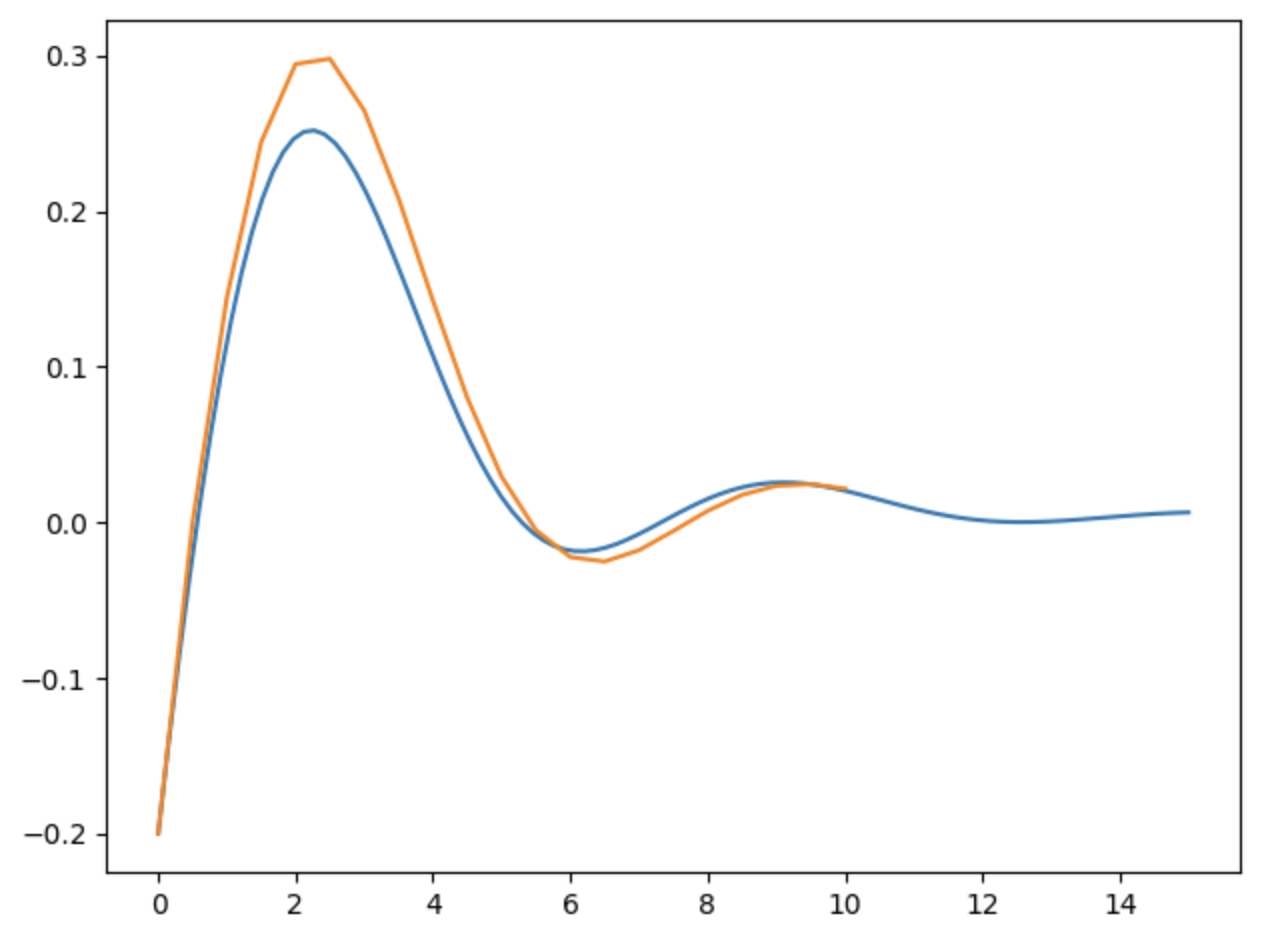
\includegraphics[scale=0.35]{CaptureEquadiff03.png} 
\end{center}

\end{frame}

%%%%%%%%%%%%%%%%%%%%%%%%%%%%%%%%%%%%%%%%%%%%%%%%%%%%%%%%%%%%%%%



\begin{frame}[fragile]
 \frametitle{Exemple: Méthode d'Euler améliorée}
Examinons le même problème avec la méthode d'Euler améliorée. C'est une méthode à un pas est définie par la fonction:
\[\myredbox{\Phi(t,z,h)=F(t+\frac h{2},z+\frac h{2} F(t,z))}\]
\begin{minted}[
mathescape,
framesep=2mm,
baselinestretch=1.2,
fontsize=\footnotesize,
linenos
]{python}
def Phi(t,y,h):
    return F(t+h/2,y+h/2*F(t,y))
    
# Méthode d'Euler améliorée $\Phi(t,z,h)=F(t+\frac{h}{2},z+\frac{h}{2} F(t,z))$
def eulerAmelioree(Phi,a,b,y0,n):
    h=(b-a)/n
    y=np.zeros(n+1)
    y[0]=y0
    t = np.linspace(a, b, n+1)
    for k in range(n):
        y[k+1]=y[k]+h*Phi(t[k],y[k],h)
    return t,y

\end{minted}

\end{frame}
%%%%%%%%%%%%%%%%%%%%%%%%%%%%%%%%%%%%%%%%%%%%%%%%%%%%%%%%%%%%%%%




\begin{frame}[fragile]
\begin{minted}[
mathescape,
framesep=2mm,
baselinestretch=1.2,
fontsize=\footnotesize,
linenos
]{python}
X,Y = eulerAmelioree(Phi,0,10,-1/5,20)
x=np.linspace(0,15,100)
y=f(x)
plt.plot(x,f(x),color='blue') # courbe exacte
plt.plot(X,Y,color='orange')    # solution approchée
plt.show()
\end{minted}

\begin{center}
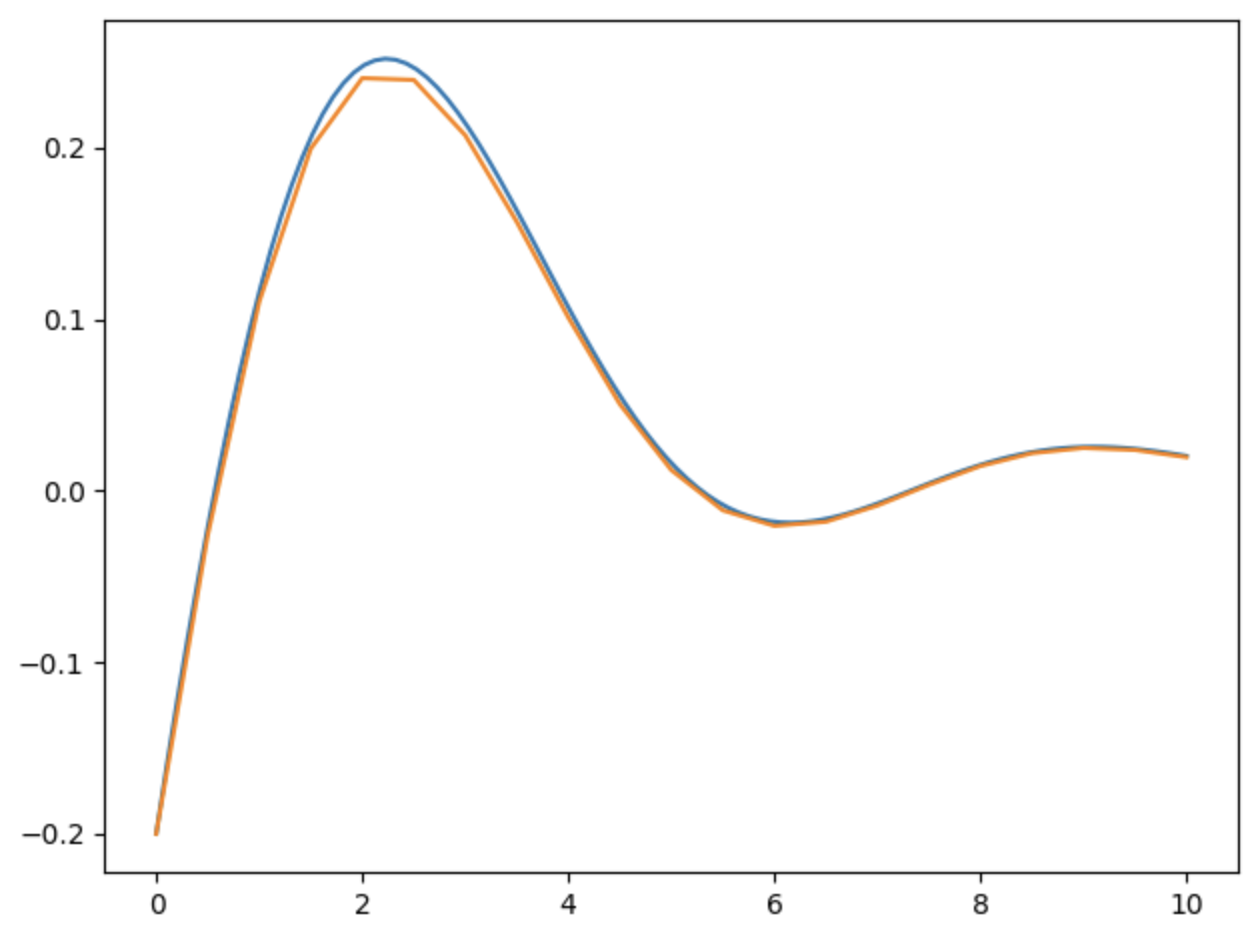
\includegraphics[scale=0.35]{CaptureEquadiff05.png} 
\end{center}
 \end{frame}
 
 %%%%%%%%%%%%%%%%%%%%%%%%%%%%%%%%%%%%%%%%%%%%%%%%%%%%%%%%%%%%%%%

\begin{frame}[fragile]
\frametitle{La méthode de Runge-Kutta}
\begin{minted}[
mathescape,
framesep=2mm,
baselinestretch=1.2,
fontsize=\footnotesize,
linenos
]{python}
def rk4(Phi,a,b,y0,n):
    h=(b-a)/n
    y=np.zeros(n+1)
    y[0]=y0
    t = np.linspace(a, b, n+1)
    for k in range(n):
        K1=F(t[k],y[k])
        K2=F(t[k]+h/2,y[k]+h/2*K1)
        K3 = F(t[k] + h / 2, y[k] + h / 2 * K2)
        K4 = F(t[k] + h , y[k] + h * K3)
        y[k+1]=y[k]+h*(K1+2*K2+2*K3+K4)/6
    return t,y

X,Y = rk4(F,0,10,-1/5,20)
x=np.linspace(0,15,100)
plt.plot(x,f(x),color='blue') # courbe exacte
plt.plot(X,Y,color='orange')    # solution approchée
plt.show()
\end{minted}
\end{frame}
 
  %%%%%%%%%%%%%%%%%%%%%%%%%%%%%%%%%%%%%%%%%%%%%%%%%%%%%%%%%%%%%%%
 
 \begin{frame}
 \frametitle{La méthode de Runge-Kutta}
\begin{center}
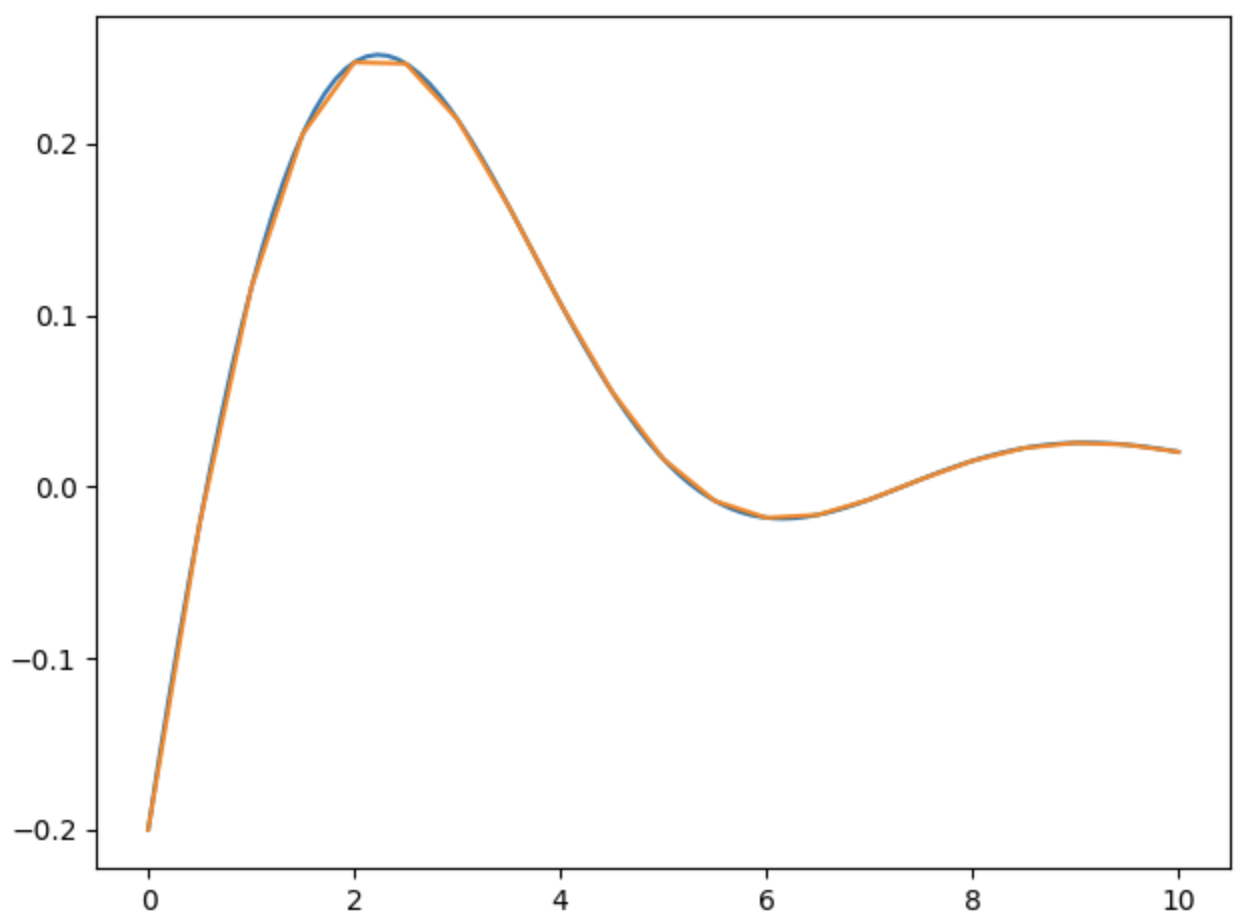
\includegraphics[scale=0.35]{CaptureEquadiff07.png} 
\end{center}

 \end{frame}
 
  %%%%%%%%%%%%%%%%%%%%%%%%%%%%%%%%%%%%%%%%%%%%%%%%%%%%%%%%%%%%%%%

 
 %%%%%%%%%%%%%%%%%%%%%%%%%%%%%%%%%%%%%%%%%%%%%%%%%%%%%%%%%%%%%%%
 \begin{frame}
 \frametitle{Exemple: Chute libre}
  On lance un projectile de masse $m$ avec une vitesse initiale $\vec{v_0}$ verticale. L'axe vertical $(O;y)$ est orienté vers le bas.
\begin{center}
 \begin{tikzpicture}[scale=0.5]
  \draw[->] (-0.1,0) -- (7.5,0)  node[right] {$\scriptstyle x$};
  \draw[->] (0,0.1) -- (0,-6) node[below] {$\scriptstyle y$};
   \draw[orange,dotted]  (0,-5.5) -- (7,-5.5) ;
   \draw[orange,dotted]  (7,0) -- (7,-5.5) ;
   \path[fill=gray]  (3.50,-1.5) circle (1.5mm) ;

   %\draw [domain=0:5][line width=0.5] plot(\x,{-1-(\x-2)^2/2});

\end{tikzpicture}
 \end{center}

 L'équation différentielle du mouvement $\frac{\de^2 M}{\de t^2}=\vec g$ s'écrit  : 
  \[
  y''=g
\]
  
  \end{frame}
 %%%%%%%%%%%%%%%%%%%%%%%%%%%%%%%%%%%%%%%%%%%%%%%%%%%%%%%%%%%%%%%
 \begin{frame}
 \frametitle{Exemple: Chute libre}
  

  On pose $z_0=y$, $z_1=y'$. On a alors
  \[\left\{\begin{array}{l}
  z_0'=z_1\\
  z_1'=g
  \end{array}\right.\]
  
     On a donc un problème de Cauchy:
  \[\left\{\begin{array}{l}
  Z'=f(t,Z)\\
  Z_0 \mbox{ donné}
  \end{array}\right.\]
  où $Z=[z_0,z_1]$, $f(t,Z)=[z_1,g]$ et $Z_0=[y_0,-v_0]$
  
  Le schéma d'Euler s'écrit:
  
  \[\left\{\begin{array}{l}
  Z_{k+1}=Z_k+h\,f(t_k,Z_k)\\
  Z_0 =[600,-100]
  \end{array}\right.\]
  où $h=0.1s$ et $g=9.81 m/s^2$.
  
  \end{frame}
 %%%%%%%%%%%%%%%%%%%%%%%%%%%%%%%%%%%%%%%%%%%%%%%%%%%%%%%%%%%%%%%

\begin{frame}[fragile]

\begin{minted}[
mathescape,
%frame=lines,
framesep=2mm,
baselinestretch=1.2,
%bgcolor=LightGray,
fontsize=\footnotesize,
linenos
]{python}
from tkinter import *
import numpy as np
# coordonnees initiales $(x_0,y_0)$
x0, y0 = 10, 200
# vitesse initiale: angle de tir $\alpha$ et vitesse $v_0$
alpha=np.pi/3 ; V0=50
h=0.1 # pas du temps
z=np.array([x0,y0,V0*np.cos(alpha),-V0*np.sin(alpha)])
def f(z):
    return np.array([z[2],z[3],0,9.81])

def Euler():
    global z
    z=z+h*f(z)
    # deplacement de la balle a la nouvelle position
    can1.coords(balle, z[0], z[1], z[0] + 30, z[1] + 30)
    # La fenetre fen1 est actualisee en executant la
    # fonction Euler toutes les 10 millisecondes
    fen1.after(10, Euler)
\end{minted}
\end{frame}
%%%%%%%%%%%%%%%%%%%%%%%%%%%%%%%%%%%%%%%%%%%%%%%%%%%%%%%%%%%%%%%

\begin{frame}[fragile]

\begin{minted}[
%frame=lines,
framesep=2mm,
baselinestretch=1.2,
%bgcolor=LightGray,
fontsize=\footnotesize,
linenos
]{python}

# ========== Programme principal =============
# Creation de la fenetre principale :
fen1 = Tk()
fen1.title("Chute libre")
# creation du canvas :
H=W=750
can1 = Canvas(fen1, bg="dark grey", height=H, width=W)
can1.pack()
# creation de la balle
balle = can1.create_oval(x0, y0, x0 + 30, y0 + 30, width=2, fill="red")
# Lancement de la fonction Euler
Euler()
# demarrage de la boucle principale:
fen1.mainloop()
\end{minted}
\end{frame}
 %%%%%%%%%%%%%%%%%%%%%%%%%%%%%%%%%%%%%%%%%%%%%%%%%%%%%%%%%%%%%%%
 \begin{frame}
 \frametitle{Exemple: Problème de tir}
  On lance un projectile de masse $m$ avec une vitesse initiale $\vec{v_0}$ faisant un angle $\alpha$ avec l'axe horizontale. Le plan de tir est porté par un système d'axes $(O;x,y)$.
\begin{center}
 \begin{tikzpicture}[scale=0.5]
  \draw[->] (-0.1,0) -- (7.5,0)  node[right] {$\scriptstyle x$};
  \draw[->] (0,0.1) -- (0,-6) node[below] {$\scriptstyle y$};
   \draw[orange,dotted]  (0,-5.5) -- (7,-5.5) ;
   \draw[orange,dotted]  (7,0) -- (7,-5.5) ;
   \path[fill=black]  (1,-1.5) circle (1mm) [fill=gray];

   \draw [domain=0:5][line width=0.5] plot(\x,{-1-(\x-2)^2/2});

\end{tikzpicture}
 \end{center}

 L'équation différentielle du mouvement $\frac{\de^2 M}{\de t^2}=\vec g$ s'écrit  en coordonnées $x$, $y$ de M: 
  \[\left\{\begin{array}{l}
  x''=0\\
  y''=g
  \end{array}\right.\]
  
  \end{frame}
 %%%%%%%%%%%%%%%%%%%%%%%%%%%%%%%%%%%%%%%%%%%%%%%%%%%%%%%%%%%%%%%
 \begin{frame}
 \frametitle{Exemple: Problème de tir}
  

  On pose $z_0=x$, $z_1=y$, $z_2=x'$,$z_3=y'$. On a alors
  \[\left\{\begin{array}{l}
  z_0'=z_2\\
  z_1'=z_3\\
  z_2'=0\\
  z_3'=g
  \end{array}\right.\]
  
     On a donc un problème de Cauchy:
  \[\left\{\begin{array}{l}
  Z'=f(t,Z)\\
  Z_0 \mbox{ donné}
  \end{array}\right.\]
  où $Z=[z_0,z_1,z_2,z_3]$, $f(t,Z)=[z_2,z_3,0,g]$ et $Z_0=[x_0,y_0,v_0\cos(\alpha),-v_0\sin(\alpha)]$
  
  Le schéma d'Euler s'écrit:
  
  \[\left\{\begin{array}{l}
  Z_{k+1}=Z_k+h\,f(t_k,Z_k)\\
  Z_0 =[10,200,50\cos(\pi/3),-50\sin(\pi/3)]
  \end{array}\right.\]
  où $h=0.1s$ et $g=9.81 m/s^2$.
  
  
  
\end{frame}

 %%%%%%%%%%%%%%%%%%%%%%%%%%%%%%%%%%%%%%%%%%%%%%%%%%%%%%%%%%%%%%%

\begin{frame}[fragile]

\begin{minted}[
%frame=lines,
framesep=2mm,
baselinestretch=1.2,
%bgcolor=LightGray,
fontsize=\footnotesize,
linenos
]{python}
from tkinter import *
import numpy as np
H=W=750
# coordonnées initiales
x0,y0=W/2,600
# vitesse initiale
V0=100
h=0.05
z=np.array([y0,-V0])
# équadiff: y'=f(t,y)
def f(y):
    return np.array([z[1],9.81])
def Euler():
    global z
    z = z + h * f(z)
    # position de la balle
    can1.coords(balle,x0,z[0],x0+30,z[0]+30)
    fen1.after(10,Euler)

\end{minted}
\end{frame}
%%%%%%%%%%%%%%%%%%%%%%%%%%%%%%%%%%%%%%%%%%%%%%%%%%%%%%%%%%%%%%%

\begin{frame}[fragile]

\begin{minted}[
%frame=lines,
framesep=2mm,
baselinestretch=1.2,
%bgcolor=LightGray,
fontsize=\footnotesize,
linenos
]{python}

#========= Programme principal ============
fen1 = Tk()
fen1.title("Problème de tir")
can1 =Canvas(fen1, bg='dark grey',height=H,width=W)
can1.pack()
balle = can1.create_oval(x0,y0,x0+30,y0+30,width=2,fill='red')
Euler()
fen1.mainloop()
\end{minted}
\end{frame}
%%%%%%%%%%%%%%%%%%%%%%%%%%%%%%%%%%%%%%%%%%%%%%%%%%%%%%%%%%%%%%%%%
\begin{frame}
\begin{center}
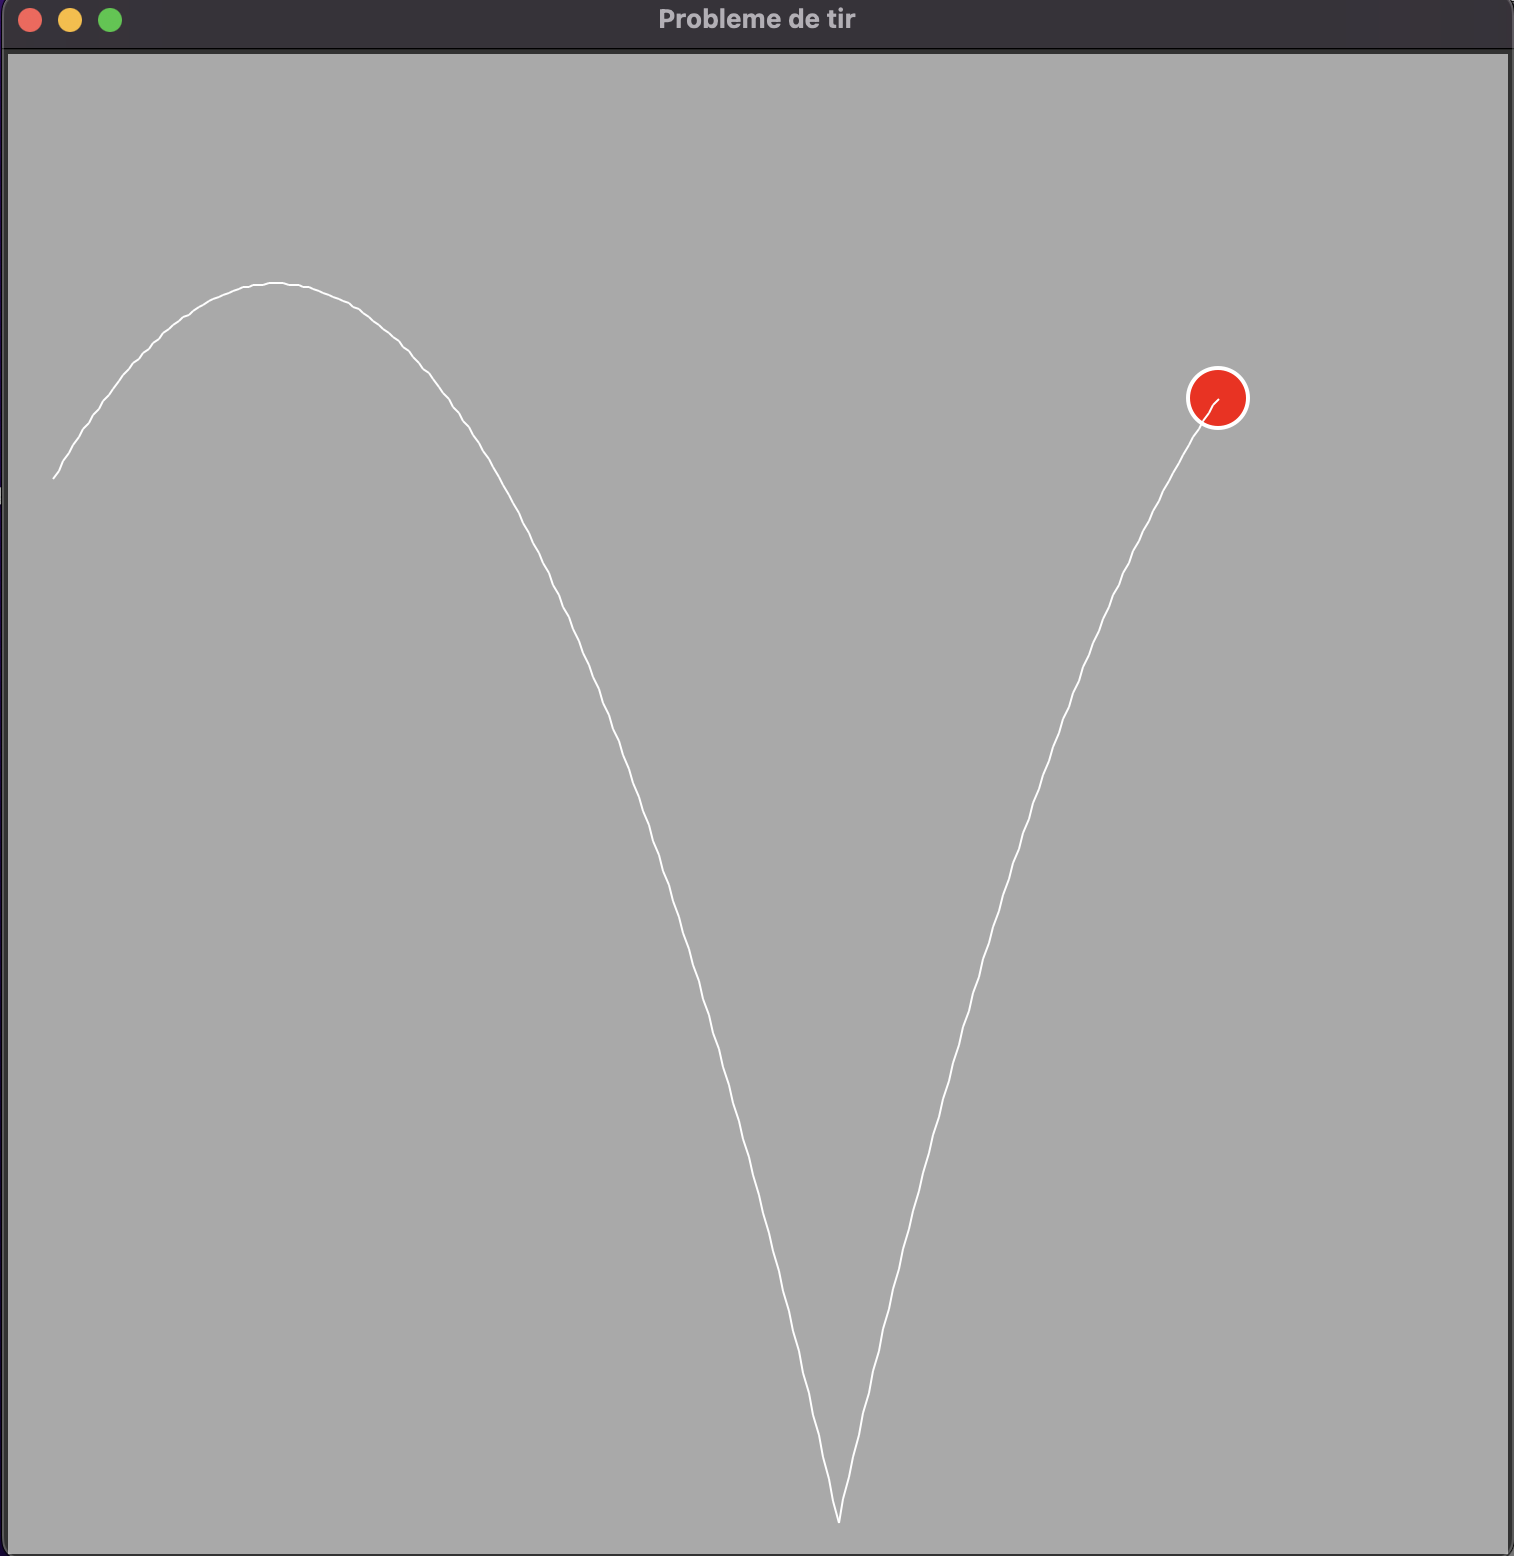
\includegraphics[scale=0.30]{images/codePbmDeTir03.png} 
\end{center}

\end{frame}

  \end{document}
   

























